\documentclass{llncs}
\usepackage{amssymb}
\usepackage{graphicx}
\usepackage[ruled,linesnumbered,boxed]{algorithm2e}
\usepackage{graphicx}
\usepackage{amsmath}
%\usepackage{mathtools}
%\usepackage{color}
\usepackage{tabularx}
\usepackage[colorlinks, linkcolor=blue, anchorcolor=blue, citecolor=green]{hyperref}
%\usepackage{booktabs}
\usepackage[table]{xcolor}
%\uespackage{colortbl}
\usepackage[tight,footnotesize]{subfigure}
\usepackage{fancyhdr}
\usepackage{lastpage}
\usepackage{layout}
\usepackage{booktabs}
\usepackage{float}
\usepackage{minted}
%\usepackage{ctex}

%\footskip = 10pt
\pagestyle{fancy}
\chead{Group Project}
\lhead{CS214-Algorithm@SJTU}
\rhead{Instructor: Xiaofeng Gao}
\rfoot{}
\cfoot{Page \thepage \ of \pageref{LastPage}}
\addtolength{\headheight}{0.5\baselineskip}
\addtolength{\headwidth}{0\marginparsep}
\addtolength{\headwidth}{0\marginparwidth}


\title{Online Ride-Hailing Platform}
\subtitle{The Sub-Title of Your Project \vspace{-3mm}}

\author{Tian Bai (119033910132, 919600234@qq.com), Christopher Harth-Kitzerow (J11903099005, c.harth-kitzerow@gmx.de), Hao Chen (119039910036, 958577057@qq.com)}
\institute{Department of Computer Science, \\ Shanghai Jiao Tong University, Shanghai, China}

\begin{document}
\bibliographystyle{splncs}

%\linespread{0.85}

%==============================================================================
\maketitle
\begin{abstract}\vspace{-5mm}
This report is our design of the the Online Ride-Hailing Platform. Considering the current situations of online ride-hailing, we have given two kinds of assignment schema. One is just the redescription of the \textit{Assignment Problem}, for which the Hungarian Algorithm can give an optimal solution. The algorithm has polynomial time complexity, and we have given an implement of the Hungarian Algorithm with time complexity of $O(n^4)$. The other is similar with the \textit{Minimum Makespan Scheduling Problem}, which is NP-hard, and we have designed an approximation algorithm for it, but the approximation ratio remains to be determined. For the future unmanned vehicles, based on our approximation algorithm and the real data, we designed an algorithm to learn from historical data, which tries to optimize the locations of the unmanned vehicles. At the end of this report, we showed our results of simulation, which illustrated that our algorithm had improved the assignments of vehicles with orders.

\textbf{Keywords:} Online Ride-Hailing, Assignment Problem, Hungarian Algorithm, Approximation Algorithm, Simulation.
\end{abstract}

\section{Ride-Hailing Problem}
There are $m$ vehicles and $n$ orders, and the distance from vehicle $i$ to order $j$ is $d_{ij}$.

\subsection{An One-to-One Version}
Suppose one vehicle can be dispatched to one and only one order. The goal is to find a dispatch handling as many orders as possible with minimum sum of distances.

When the driver of the vehicle is a man, this situation is very common because after the vehicle arriving the destination of the order, the driver prefers to picking up passengers around the destination.

\subsection{An One-to-Many Version}
Suppose when one vehicle has finished an order, it will go back to its original location. The goal is to find a dispatch handling all orders with minimum maximum sum of distances for picking up passengers of all vehicles.

The supposition is based on the fact that the destination of an order may be stochastic, it is hard to include the distance from hailing place to destination. Or we can just assume these distances are equal for all orders, however, this has no differences with ignoring them for finding the minumum maximum sum of distances.

This is a generalization of the \textit{Minimum Makespan Scheduling Problem} (just need to assume all vehicle are at same location), and the latter is NP-hard (can be proved by a reduction from \textit{Subset Sum Problem}). Therefore, our problem is NP-hard.

\section{Algorithm Design}

\subsection{Hungarian Algorithm}
Let's recall the \textit{Assignment Problem}\cite{assignment_problem_wiki}: There are a number of agents and a number of tasks. Any agent can be assigned to perform any task, incurring some cost that may vary depending on the agent-task assignment. It is required to perform as many tasks as possible by assigning at most one agent to each task and at most one task to each agent, in such a way that the total cost of the assignment is minimized.

From above description, we can see our \textit{One-to-One Version} is equivalent to the \textit{Assignment Problem}. We can suppose $m=n$, otherwise, we can easily add some vehicles or orders whose distances to any orders or vehicles are zero. After this, we can use Hungarian Algorithm\cite{hungarian_algorithm_wiki,hungarian_algorithm} to solve it, whose time complexity is $O(n^4)$.

The Hungarian Algorithm consists of the four steps below. The first two steps are executed once, while steps 3 and 4 are repeated until an optimal assignment is found. The input of the algorithm is an $n$ by $n$ square matrix with only nonnegative elements.

\begin{itemize}
    \item Step 1: Subtract row minima \\
    For each row, find the lowest element and subtract it from each element in that row.
    \item Step 2: Subtract column minima \\
    Similarly, for each column, find the lowest element and subtract it from each element in that row.
    \item Step 3: Cover all zeros with minimum numbers of lines \\
    Cover all zeros in the resulting matrix using minimum number of horizontal and vertical lines. If $n$ lines are required, an optimal assignment exists among the zeros. The algorithm stops. \\
    If less than $n$ lines are required, continue with Step 4.
    \item Step 4: Create additional zeros \\
    Find the smallest element (call it $k$) that is not covered by a line in Step 3. Subtract $k$ from all uncovered elements, and add $k$ to all elements that are covered twice. Go to Step 3.
\end{itemize}

We consider an example where for four jobs (J1, J2, J3 and J4) need to be executed by four workers (W1, W2, W3 and W4), one job per worker. The matrix below shows the cost of assigning a certain worker to a certain job. The objective is to minimize the total cost of the assignment.
% Table generated by Excel2LaTeX from sheet 'Sheet1'
\begin{table}[H]
  \centering
%   \caption{Add caption}
    \begin{tabular}{ccccc}
    \toprule
          & J1    & J2    & J3    & J4 \\
    \midrule
    \phantom{2333} W1 \phantom{2333}   & \phantom{2333} 82 \phantom{2333}   & \phantom{2333} 83 \phantom{2333}   & \phantom{2333} 69 \phantom{2333}   & \phantom{2333} 92 \phantom{2333} \\
    W2    & 77    & 37    & 49    & 92 \\
    W3    & 11    & 69    & 5     & 86 \\
    W4    & 8     & 9     & 98    & 23 \\
    \bottomrule
    \end{tabular}%
%   \label{tab:addlabel}%
\end{table}%

\textbf{Step 1: Substrac row minima}

We start with subtracting the row minimum from each row. The smallest element in the first row is, for example, 69. Therefore, we substract 69 from each element in the first row. The resulting matrix is:
% Table generated by Excel2LaTeX from sheet 'Sheet1'
\begin{table}[H]
  \centering
%   \caption{Add caption}
    \begin{tabular}{cccccc}
\toprule         & J1    & J2    & J3    & J4    &  \\
\midrule   \phantom{2333} W1 \phantom{2333}   & \phantom{2333} 13 \phantom{2333}   & \phantom{2333} 14 \phantom{2333} & \phantom{2333} 0 \phantom{2333}    & \phantom{2333} 23 \phantom{2333} & \phantom{2333} (-69) \phantom{2333} \\
    W2    & 40    & 0     & 12    & 55    & (-37) \\
    W3    & 6     & 64    & 0     & 81    & (-5) \\
    W4    & 0     & 1     & 90    & 15    & (-8) \\
\bottomrule    \end{tabular}%
%   \label{tab:addlabel}%
\end{table}%

\textbf{Step 2: Subtract column minima}

Similarly, we subtract the column minimum from each column, giving the following matrix:
% Table generated by Excel2LaTeX from sheet 'Sheet1'
\begin{table}[H]
  \centering
%   \caption{Add caption}
    \begin{tabular}{ccccc}
    \toprule
          & J1    & J2    & J3    & J4 \\
    \midrule
    \phantom{2333} W1 \phantom{2333}   & \phantom{2333} 13 \phantom{2333}   & \phantom{2333} 14 \phantom{2333}   & \phantom{2333} 0 \phantom{2333}    & \phantom{2333} 8 \phantom{2333} \\
    W2    & 40    & 0     & 12    & 40 \\
    W3    & 6     & 64    & 0     & 66 \\
    W4    & 0     & 1     & 90    & 0 \\
          &       &       &       & (-15) \\
    \bottomrule
    \end{tabular}%
%   \label{tab:addlabel}%
\end{table}%

\textbf{Step 3: Cover all zeros with a minimum number of lines}

We will now determine the minimum number of lines (horizontal or vertical) that are required to cover all zeros in the matrix. All zeros can be covered using 3 lines:
% Table generated by Excel2LaTeX from sheet 'Sheet1'
\begin{table}[H]
  \centering
%   \caption{Add caption}
    \begin{tabular}{cccccc}
    \toprule
          & J1    & J2    & J3    & J4    &  \\
    \midrule
    \phantom{2333} W1 \phantom{2333}   & \phantom{2333} 13 \phantom{2333}   & \phantom{2333} 14 \phantom{2333}   & \cellcolor[rgb]{ 0,  .69,  .941} \phantom{2333} 0 \phantom{2333} & \phantom{2333} 8 \phantom{2333}    & \phantom{2333} \phantom{x} \phantom{2333} \\
    W2    & \cellcolor[rgb]{ 0,  .69,  .941}40 & \cellcolor[rgb]{ 0,  .69,  .941}0 & \cellcolor[rgb]{ 0,  .69,  .941}12 & \cellcolor[rgb]{ 0,  .69,  .941}40 & x \\
    W3    & 6     & 64    & \cellcolor[rgb]{ 0,  .69,  .941}0 & 66    &  \\
    W4    & \cellcolor[rgb]{ 0,  .69,  .941}0 & \cellcolor[rgb]{ 0,  .69,  .941}1 & \cellcolor[rgb]{ 0,  .69,  .941}90 & \cellcolor[rgb]{ 0,  .69,  .941}0 & x \\
          &       &       & x     &       &  \\
    \bottomrule
    \end{tabular}%
%   \label{tab:addlabel}%
\end{table}%

Because the number of lines required (3) is lower than the size of the matrix (n=4), we continue with Step 4.

\textbf{Step 4: Create additional zeros}

First, we find that the smallest uncovered number is 6. We subtract this number from all uncovered elements and add it to all elements that are covered twice. This results in the following matrix:
% Table generated by Excel2LaTeX from sheet 'Sheet1'
\begin{table}[H]
  \centering
%   \caption{Add caption}
    \begin{tabular}{ccccc}
    \toprule
          & J1    & J2    & J3    & J4 \\
    \midrule
    \phantom{2333} W1 \phantom{2333}   & \phantom{2333} 7 \phantom{2333}    & \phantom{2333} 8 \phantom{2333}    & \phantom{2333} 0 \phantom{2333}    & \phantom{2333} 2 \phantom{2333}\\
    W2    & 40    & 0     & 18    & 40 \\
    W3    & 0     & 58    & 0     & 60 \\
    W4    & 0  & 1     & 96    & 0 \\
    \bottomrule
    \end{tabular}%
%   \label{tab:addlabel}%
\end{table}%

Now we return to Step 3.

\textbf{Step 3: Cover all zeros with a minimum number of lines}

Again, We determine the minimum number of lines required to cover all zeros in the matrix. Now there are 4 lines required:
% Table generated by Excel2LaTeX from sheet 'Sheet1'
\begin{table}[H]
  \centering
%   \caption{Add caption}
    \begin{tabular}{cccccc}
    \toprule
          & J1    & J2    & J3    & J4    &  \\
    \midrule
    \phantom{2333} W1 \phantom{2333}   & \cellcolor[rgb]{ 0,  .69,  .941}\phantom{2333} 7 \phantom{2333} & \cellcolor[rgb]{ 0,  .69,  .941}\phantom{2333} 8 \phantom{2333} & \cellcolor[rgb]{ 0,  .69,  .941}\phantom{2333} 0 \phantom{2333} & \cellcolor[rgb]{ 0,  .69,  .941}\phantom{2333} 2 \phantom{2333} & \phantom{2333} x \phantom{2333} \\
    W2    & \cellcolor[rgb]{ 0,  .69,  .941}40 & \cellcolor[rgb]{ 0,  .69,  .941}0 & \cellcolor[rgb]{ 0,  .69,  .941}18 & \cellcolor[rgb]{ 0,  .69,  .941}40 & x \\
    W3    & \cellcolor[rgb]{ 0,  .69,  .941}0 & \cellcolor[rgb]{ 0,  .69,  .941}58 & \cellcolor[rgb]{ 0,  .69,  .941}0 & \cellcolor[rgb]{ 0,  .69,  .941}60 & x \\
    W4    & \cellcolor[rgb]{ 0,  .69,  .941}0 & \cellcolor[rgb]{ 0,  .69,  .941}1 & \cellcolor[rgb]{ 0,  .69,  .941}96 & \cellcolor[rgb]{ 0,  .69,  .941}0 & x \\
    \bottomrule
    \end{tabular}%
%   \label{tab:addlabel}%
\end{table}%

Because the number of lines required (4) equals the size of the matrix (n=4), an optimal assignment exists among the zeros in the matrix. Therefore, the algorithm stops.

\textbf{The optimal assignment}

The following zeros cover an optimal assignment:
% Table generated by Excel2LaTeX from sheet 'Sheet1'
\begin{table}[H]
  \centering
%   \caption{Add caption}
    \begin{tabular}{ccccc}
    \toprule
          & J1    & J2    & J3    & J4 \\
    \midrule
    \phantom{2333} W1 \phantom{2333}   & \phantom{2333} 7 \phantom{2333}    & \phantom{2333} 8 \phantom{2333}    & \cellcolor[rgb]{ 0,  .69,  .941}\phantom{2333} 0 \phantom{2333} & \phantom{2333} 2 \phantom{2333} \\
    W2    & 40    & \cellcolor[rgb]{ 0,  .69,  .941}0 & 18    & 40 \\
    W3    & \cellcolor[rgb]{ 0,  .69,  .941}0 & 58    & 0     & 60 \\
    W4    & 0     & 1     & 96    & \cellcolor[rgb]{ 0,  .69,  .941}0 \\
    \bottomrule
    \end{tabular}%
%   \label{tab:addlabel}%
\end{table}%

This corresponds to the following optimal assignment in the original cost matrix:
% Table generated by Excel2LaTeX from sheet 'Sheet1'
\begin{table}[H]
  \centering
%   \caption{Add caption}
    \begin{tabular}{ccccc}
    \toprule
          & J1    & J2    & J3    & J4 \\
    \midrule
    \phantom{2333} W1 \phantom{2333}   & \phantom{2333} 82 \phantom{2333}   & \phantom{2333} 83 \phantom{2333}   & \cellcolor[rgb]{ 0,  .69,  .941}\phantom{2333} 69 \phantom{2333} & \phantom{2333} 92 \phantom{2333}\\
    W2    & 77    & \cellcolor[rgb]{ 0,  .69,  .941}37 & 49    & 92 \\
    W3    & \cellcolor[rgb]{ 0,  .69,  .941}11 & 69    & 5     & 86 \\
    W4    & 8     & 9     & 98    & \cellcolor[rgb]{ 0,  .69,  .941}23 \\
    \bottomrule
    \end{tabular}%
%   \label{tab:addlabel}%
\end{table}%

Thus, worker 1 should perform job 3, worker 2 job 2, worker 3 job 1, and worker 4 should perform job 4. The total cost of this optimal assignment is to $69 + 37 + 11 + 23 = 140$.

\subsection{Approximation Algorithm}
The Approximation Algorithm is designed to solve the \textit{One-to-Many Version}, whose idea is from the approximation algorithm of the \textit{Minimum Makespan Scheduling Problem}. The detail is as follows:

\begin{minipage}[t]{0.8\textwidth}
\begin{algorithm}[H]
	\BlankLine
	\SetKwInOut{Input}{input}
	\SetKwInOut{Output}{output}
	\caption{Local Assignment}\label{Alg_Local_Assignment}
	\Input{$m$ vehicles, $n$ orders and distances matrix $D_{m\times n}$.}
	\Output{An assignment for all orders.}
	\BlankLine
	Let $S$ be an arbitrary assignment\;
	
	\Repeat{There doesn't exist any above reassignment}{
	    Consider the order $l$ leading to the maximum sum of distances\;
	    Find a vehicle $k$, when reassigning $l$ to $k$, the sum of distances for $k$ is minimal in all vehicles\;
	}
	
	\Return{$S$}\;
	
\end{algorithm}
\end{minipage}

We consider an example where for six jobs (J1, J2, J3, J4, J5 and J6) need to be executed by four workers (W1, W2, W3 and W4). The matrix below shows the cost of assigning a certain worker to a certain job. The objective is to minimize the maximum sum of costs of all works.
% Table generated by Excel2LaTeX from sheet 'Sheet1'
\begin{table}[H]
  \centering
%   \caption{Add caption}
    \begin{tabular}{ccccccc}
    \toprule
          & J1    & J2    & J3    & J4    & J5    & J6 \\
    \midrule
    \phantom{2333} W1 \phantom{2333}    & \phantom{2333} 82 \phantom{2333}   & \phantom{2333} 83 \phantom{2333}    & \phantom{2333} 69 \phantom{2333}   & \phantom{2333} 92 \phantom{2333}   & \phantom{2333} 47 \phantom{2333}    & \phantom{2333} 87 \phantom{2333} \\
    W2    & 77    & 37    & 49    & 92    & 56    & 7 \\
    W3    & 11    & 69    & 5     & 86    & 19    & 66 \\
    W4    & 8     & 9     & 98    & 23    & 22    & 42 \\
    \bottomrule
    \end{tabular}%
%   \label{tab:addlabel}%
\end{table}%

% Table generated by Excel2LaTeX from sheet 'Sheet1'
\begin{table}[H]
  \centering
%   \caption{Add caption}
\begin{minipage}[t]{0.45\textwidth}
    \centering
    \begin{tabular}{ccc}
    \toprule
          & Jobs  & Cost \\
    \midrule
    \phantom{2333} W1 \phantom{2333}   & \phantom{2333} J1, J2 \phantom{2333} & \phantom{2333} 165 \phantom{2333} \\
    W2    & J3, J4 & 141 \\
    W3    & J5    & 19 \\
    W4    & J6    & 42 \\
    \bottomrule
    \end{tabular}%
    \vskip .5em
    (1)
\end{minipage}
%   \label{tab:addlabel}%
%%
\begin{minipage}[t]{0.45\textwidth}
    \centering
    \begin{tabular}{ccc}
    \toprule
          & Jobs  & Cost \\
    \midrule
    \phantom{2333} W1 \phantom{2333}   & \phantom{2333} J1 \phantom{2333}   & \phantom{2333} 82 \phantom{2333}\\
    W2    & J3, J4 & 141 \\
    W3    & J5    & 19 \\
    W4    & J6, J2 & 51 \\
    \bottomrule
    \end{tabular}%
    \vskip .5em
    (2)
\end{minipage}
\end{table}%

% Table generated by Excel2LaTeX from sheet 'Sheet1'
\begin{table}[H]
  \centering
%   \caption{Add caption}
\begin{minipage}[t]{0.45\textwidth}
    \centering
    \begin{tabular}{ccc}
    \toprule
          & Jobs  & Cost \\
    \midrule
    \phantom{2333} W1 \phantom{2333}   & \phantom{2333xx} J1 \phantom{xx2333}   & \phantom{2333} 82 \phantom{2333}\\
    W2    & J3    & 49 \\
    W3    & J5    & 19 \\
    W4    & J6, J2, J4 & 74 \\
    \bottomrule
    \end{tabular}%
    \vskip .5em
    (3)
\end{minipage}
%   \label{tab:addlabel}%
%%
\begin{minipage}[t]{0.45\textwidth}
    \centering
    \begin{tabular}{ccc}
    \toprule
          & Jobs  & Cost \\
    \midrule
    \phantom{2333} W1 \phantom{2333}   &    \phantom{2333xxx} \phantom{x2333}   & \phantom{2333} 0 \phantom{2333}\\
    W2    & J3    & 49 \\
    W3    & J5, J1 & 30 \\
    W4    & J6, J2, J4 & 74 \\
    \bottomrule
    \end{tabular}%
    \vskip .5em
    (4)
\end{minipage}
\end{table}%

As is shown above, (1) is an arbitrary assignment, which leads to a maximum cost of 165. Then, we try to decrease it, and we try to reassign J2 to W2, W3, W4, we have the cost of 178, 88, 51, respectively. As 51 is minimal, the final reassignment is to W4, shown in (2). We repeat these steps until there doesn't exist any reassignment. Finally, we get the local optimal cost of 74.


\section{Simulation}
\subsection{Algorithm}
With historical data, we can find a better locations for vehicles. We can set the vehicle located at the center of the orders handled by it historically, then, we can repeat the optimization. This is shown below.
\begin{minipage}[t]{0.8\textwidth}
\begin{algorithm}[H]
	\BlankLine
	\SetKwInOut{Input}{input}
	\SetKwInOut{Output}{output}
	\caption{Local Assignment with Dynamic Locations}\label{Alg_Local_Assignment_2}
	\Input{number of vehicles $m$, $n$ orders with locations.}
	\Output{An assignment for all orders.}
	\BlankLine
	\If{There doesn't exist historical data}{
	    Choose random locations for all vehicles\;
	} \Else{
	    Set all vehicles located at the center of the historical orders handled by them, respectively\;
	}
	Let $S$ be an arbitrary assignment\;
	
	\Repeat{There doesn't exist any above reassignment}{
	    Consider the order $l$ leading to the maximum sum of distances\;
	    Find a vehicle $k$, when reassigning $l$ to $k$, the sum of distances for $k$ is minimal in all vehicles\;
	}
	
	\Return{$S$}\;
	
\end{algorithm}
\end{minipage}

\subsection{Experiment Setting}
We use the NYC Taxi & Limousine Commission (TLC) data for our experiment, which is on \url{https://github.com/fivethirtyeight/uber-tlc-foil-response/tree/master/uber-trip-data}. The specifit data we use is \texttt{uber-raw-data-sep14.csv}.
% Table generated by Excel2LaTeX from sheet 'uber-raw-data-sep14'
\begin{table}[H]
  \centering
  \caption{Uber TLC Raw Data Sep. 2014 Demo}
    \begin{tabular}{cccc}
    \toprule
    Date/Time & Lat   & Lon   & Base \\
    \midrule
    \phantom{2333} 9/1/2014 0:01:00 \phantom{2333} & \phantom{2333} 40.2201 \phantom{2333}& \phantom{2333} -74.0021 \phantom{2333} & \phantom{2333} B02512 \phantom{2333} \\
    9/1/2014 0:01:00 & 40.75 & -74.0027 & B02512 \\
    9/1/2014 0:03:00 & 40.7559 & -73.9864 & B02512 \\
    9/1/2014 0:06:00 & 40.745 & -73.9889 & B02512 \\
    9/1/2014 0:11:00 & 40.8145 & -73.9444 & B02512 \\
    9/1/2014 0:12:00 & 40.6735 & -73.9918 & B02512 \\
    \bottomrule
    \end{tabular}%
  \label{tab:Uber TLC Raw Data Sep. 2014 Demo}%
\end{table}%

We just consider the orders whose bases are B01512. There are about 1100 orders per day, and we use 100 vehicles for our experiment.

\subsection{Results}
\subsubsection{Assignments}
Our program can figure out the assignments calculated by Algorithm~\ref{Alg_Local_Assignment_2}.
% Table generated by Excel2LaTeX from sheet 'Sheet1'
\begin{table}[H]
  \centering
  \caption{1 Sep. Assignments Demo}
    \begin{tabular}{ccc}
    \toprule
    vehicle & orders & distance (hm) \\
    \midrule
    0     & 27, 358 & 1145 \\
    1     & 138, 338, 413, 528, 624, 611, 557, 419, 412 & 1413 \\
    2     & 52, 74, 98, 218, 238, 264, 273, 391, 429, 492 & 1313 \\
    3     & 100, 158, 268 & 1444 \\
    4     & 137, 167, 170 & 1198 \\
    5     & 93, 102, 297, 587 & 1187 \\
    …     & …     & … \\
    \bottomrule
    \end{tabular}%
  \label{tab:1 Sep. Assignments Demo}%
\end{table}%

% Table generated by Excel2LaTeX from sheet 'Sheet1'
\begin{table}[H]
  \centering
  \caption{2 Sep. Assignments Demo}
    \begin{tabular}{ccc}
    \toprule
    vehicle & orders & distance (hm) \\
    \midrule
    0     & 206, 238, 392, 495, 719, 1003, 1085, 1107 & 639 \\
    1     & 36, 165, 167, 258, 260, 374, 399, 435 & 809 \\
    2     & 18, 183, 230, 264, 571, 705, 1013, 1031, 1042, 1123, 1175 & 761 \\
    3     & 92, 311, 319, 447, 552, 754, 822, 883, 1024, 1034, 1036, 1061, 1084, 1114, 1166 & 786 \\
    4     & 26, 38, 61, 610, 631, 747, 789, 892, 937, 1069, 861, 791, 809, 1112, 1145, 989, 846, ... & 662 \\
    5     & 57, 88, 102, 288, 417, 473, 530, 646, 764, 783, 844, 874 & 790 \\
    …     & …     & … \\
    \bottomrule
    \end{tabular}%
  \label{tab:2 Sep. Assignments Demo}%
\end{table}%

From Table~\ref{tab:1 Sep. Assignments Demo} and Table~\ref{tab:2 Sep. Assignments Demo}, we know there is a considerable difference of distances. This is due to that in the first day, we have no historical data, and we can just set locations of vehicles randomly. However, in the second day, we have used the data of the first day to set locations of vehicles. Therefore, the distance of the second day is much less than that of the first day.

\subsubsection{Distance Curve}
We have drawn the curves of distance varies with days.

\begin{figure}[H]
    \centering
    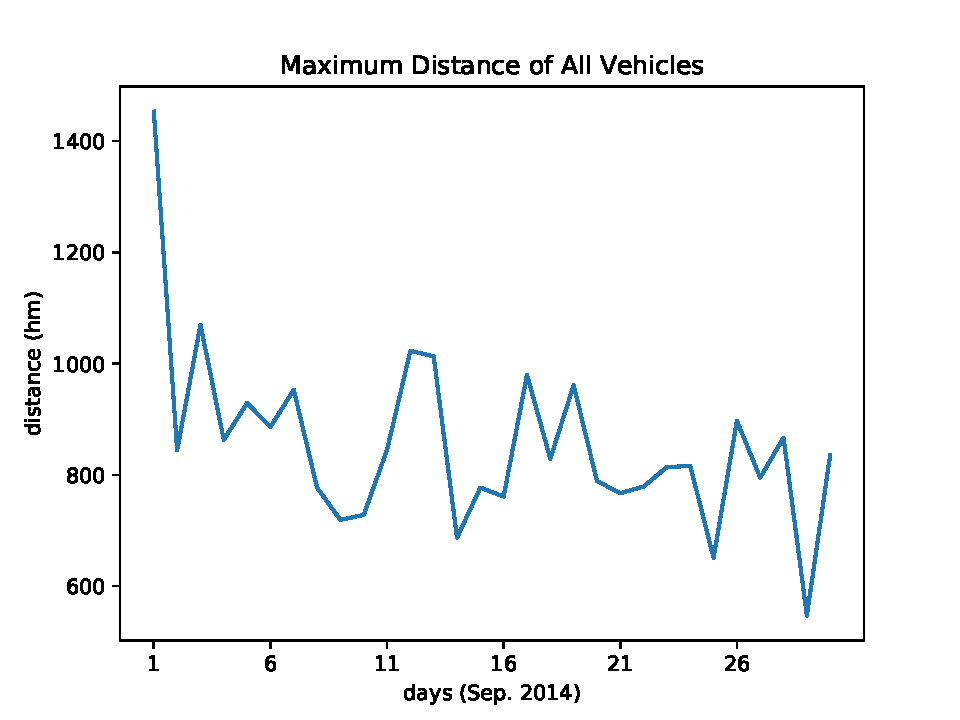
\includegraphics[width=.6\textwidth]{figures/max_distances_curve.pdf}
    \caption{Maximum Distance of All Vehicles}
    \label{fig:Maximum Distance of All Vehicles}
\end{figure}

\begin{figure}[H]
    \centering
    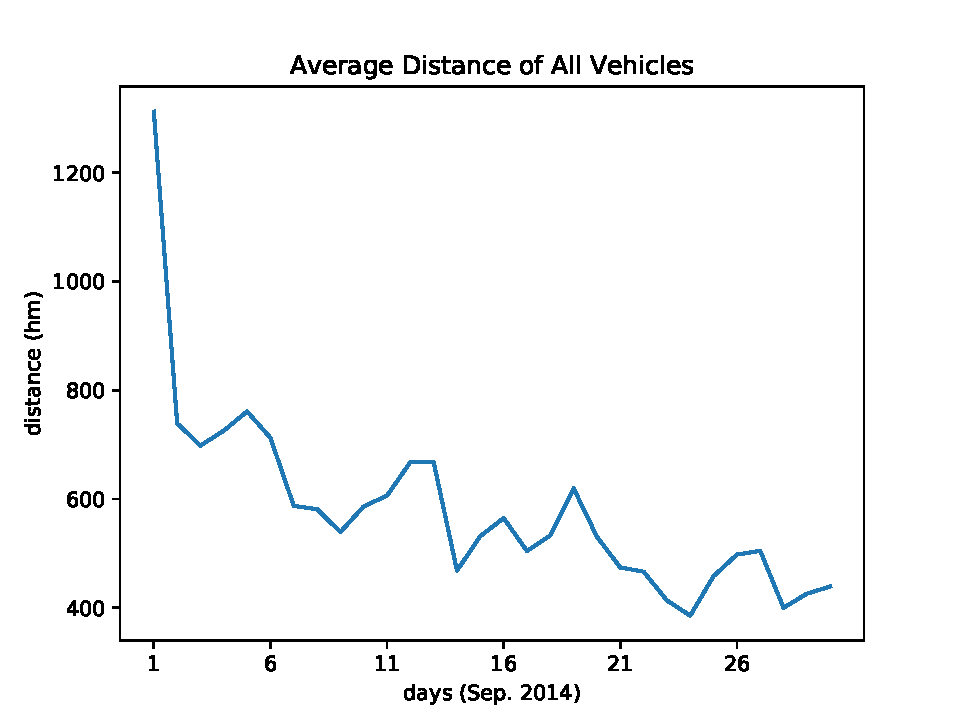
\includegraphics[width=.6\textwidth]{figures/ave_distances_curve.pdf}
    \caption{Average Distance of All Vehicles}
    \label{fig:Average Distance of All Vehicles}
\end{figure}

From Fig.~\ref{fig:Maximum Distance of All Vehicles} and Fig.~\ref{fig:Average Distance of All Vehicles}, we can see it is apparent that from 1 Sep. to 2 Sep., the distances decrease dramatically, which is similar with Table~\ref{tab:1 Sep. Assignments Demo} and Table~\ref{tab:2 Sep. Assignments Demo}. Then, for the next days, the distance decrease slowly, which suggests that our algorithm has the ability to learn from historical data and make better assignments. However, the optimization of the assignments has some limitation, which is to say, if we have thousands of historical data, it is hard for our algorithm to optimize more.

\quad\newline
\quad\newline
\quad\newline
The full results, data, source codes (include this report) can be obtained at \url{https://github.com/baitian752/online-ride-hailing-platform}.


\section*{Acknowledgements}

Firstly, I would like to give my sincere gratitude to Prof. Xiaofeng Gao, with extraordinary patience and consistent encouragement.

Secondly, I want to thank TA Wenyi Xu and Fenglin Yang, who graded our homeworks earnestly, gave us detailed solutions.

This is my first algorithm course, having given me some methods and criterions to study algorithms, making me skilled in analysing problems. After this course, I feel clear and confident with some classic problems, and I think the most important thing is that I have learned how to research some unknown problems.

Finally, I have to say, this course is difficult for most students, however, I think we just need this for our growth.

\begin{thebibliography}{9}
\bibitem{assignment_problem_wiki}
Wikipedia contributors, \url{https://en.wikipedia.org/wiki/Assignment_problem}. Last accessed 24 Dec 2019

\bibitem{hungarian_algorithm_wiki}
Wikipedia contributors, \url{https://en.wikipedia.org/wiki/Hungarian_algorithm}. Last accessed 24 Dec 2019

\bibitem{hungarian_algorithm}
Kuhn, Harold W. "The Hungarian method for the assignment problem." Naval research logistics quarterly 2.1‐2 (1955): 83-97.

\end{thebibliography}
\end{document}
